\section{Introduction}
Unmanned Aerial Vehicles (UAV) are gaining popularity in private as well as commercial sector. One often-mentioned use-case is the parcel delivery. In the near future, UAV might be used to deliver parcels to your doorstep. The logistics industry hopes for positive impacts on their costs and competitiveness. The deployment of a delivery concept is quite complex. To allow for early evaluation and reduce the number of required flight-testing, a simulation engine is required. This is why SIMULATIONNAME has been developed. It supports multiple depots and UAV as well as  simple change of path-planning algorithm. UAVs move in a 3D environment  The engine does not simulate the behaviour of the UAV in the aerial space itself but allows for evaluation of spatial distribution of depots or the suitability of a path-planning algorithm. It was developed considering the use of swarm algorithms in the delivery use-case and allow for inter-drone communication and autonomous organisation avoiding a central ground control.

\section{Related Work}
Literature on simulation engines for UAV delivery is still relatively scarce. Simulation engines that were developed concentrate rather on specific components or flight behaviour.
\cite{johnson.2001} developed a simulation engine for the behaviour of specific hardware components of a UAV. \cite{lu.2011} simulated the flight dynamic behaviour of a UAV using Matlab/Simulink. MultiUAV \cite{rasmussen.2003}, a very general simulation engine has been developed to simulate cooperative algorithms for finding targets. In 2005,  an agent-based simulation engine implementing a surveillance scenario has been developed \cite{jang.2005}. UAV try to find targets without prior knowledge of the targets’ locations. They implement UAVs as agents and also use the notion of obstacles and bases. The sensor concept is similar to the one used in this paper.

\section{Scenario}
NO CENTRAL ENTITY, optimizes
\\
Before embarking the software model, the delivery scenario shall be described.  Every UAV has a depot, in the engine called basestation, from which it receives items to be delivered. An item's destination is within the range of a Basestation which means that every Basestation has a limited range in the area. UAVs are assigned to one specific Basestation and only deliver items of it. After receiving an item, the UAV will begin flying to the specific destination. It scans the area and stores information on all fields it has seen en-route. If a UAV meets another one, they will exchange information on the already-explored parts of the area.\\
If a field on the route contains an obstacle, it will deviate from its route and try to find one around the obstacle. Obstacles can have different heights, thus UAV als\\
After delivering the item, it will fly back to the basestation to receive a new item. If the battery reaches a certain threshold, the UAV will fly to the nearest basestation (not neccessarily its home base) and recharge its battery. 
 UAVs are moving in a 3D environment which means that obstacles can have different heights.

\section{Description of the model}
The simulation has been written in Python, using the MESA framework for agent-based modelling. Figure \ref{fig:architecture} represents the software architecture. There are three major components: the simulation model itself, implementing the simulation environment and logic, an analytics interface for evaluating a simulation's performance and the GUI realized using a web server and allowing for easy access with a standard web-browser. The UAV as part of the simulation model, shall be described in particular in section \ref{sec:UAV}.\\
The simulation's aim is to support comparing of different decentralized path-planning algorithms by making them easily exchangeable. Predefined KPI's and an output method are used to support for analysing the performance of one's implementation. Section \ref{sec:KPI} discusses the way KPI's are defined.
\begin{figure}[htbp]\label{fig:architecture}
	\centering
	\includegraphics[scale=0.3]{images/architecture.png} 
	\caption{Architecture of simulation model}
\end{figure}

\begin{enumerate}
	\item General Structure :  UI, UAV Simulator, MESA, Analysis, BaseStations (depots)
	\item BaseStation: In the real world, this is the depot of a logistics company. It assigns orders to UAVs and hands items over to them. Depots are responsible for all items in a part of the map and for a subset of all drones. Also, they contain chargers for UAVs whose battery reached a low level. In the configuration, one can set how many depots are supposed to be on the map by specifying the number of fields the depot is responsible for (its delivery area). depots are located as close to the center of their area as possible, but only on obstacles (on buildings). Items that are picked up from a depot can have different priorities in order to make the simulation more realistic. For example, items with high priority can be important and immediately required medical equipment or parcels for which a customer paid a higher fee to receive it faster.
		\item An obstacle can be any static object that obstructs a UAV on its way flying to a point (such as trees, buildings etc). Obstacles can have different heights. The simulator will load the height information from a JPEG file with different colors for different heights. The height levels represent different height corridors that UAVs are allowed to fly in.
	\item 
	\item UI: GUI in Browser, config.ini: As per MESA standard, the User interface is realized using a web-server and a browser-based UI. The configuration is parsed from a configuration file,  config.ini. It configures the setup of the grid (altitude levels, pixel width/height), UAV settings such as battery life and the sensor range. The simulation also supports different runmodes, one for running unit-tests, one for ordinary run with the server and graphical user interface as well as running without GUI which improves performance as no rendering is required.
		\item Results based on predefined KPI's are written out into a CSV file to support evaluation of the simulation. Section \ref{sec:KPI} gives more information on how to work with the output file.
	\item The simulation is built upon the MESA modeling framework. The following section shall describe agent-based modelling and how it is realized using MESA.

\end{enumerate}

\subsection{MESA}
MESA \cite{masad.2015} is an open source agent-based modeling framework (ABM) developed specifically for the Python programming language.  Agents are objects that have rules and states that act accordingly on every step of the simulation \cite{axtell.2000}. ABM allows to capture the path of the simulation along with the solution and allows for analysing the dynamic history \cite{axtell.2000}. ABM also allows to dynamically pause and resume the simulation at any given step and analyse the current results.\\
MESA comes with implementations of important components, such as a grid for implementing a simple 2D environment, a web-browser-based UI, a data analysis tool and an agent scheduler. It allows for easy extension or modifications to develop specific simulation engines. \\
Our simulation uses all core components of MESA, such as the MultiGrid, the DataCollector, the scheduler (RandomActivation), agents and the server component \cite{masad.2015}:
\begin{itemize}
	\item The MultiGrid is a 2D grid with fields that allow for more than one agent on one field. This is particularly important for our simulation as agents of different height are all stored in the same grid in the model.
	\item The DataCollector is used for collecting relevant quantitative data to support the evaluation of an algorithm.
	\item The scheduler activates the agents. An agent will only do an action if the scheduler activates it. We use the RandomActivation which means that in every step the agents are activated in a random order.
	\item The server renders the graphical user interfaces and renders changes on the model. It also allows for pausing and resuming the simulation or progress step-wise. 
\end{itemize} 
\begin{itemize}
	\item Which components did we remove or modify and why?
	\item In order to optimize rendering performance, some modifications to the user interface components of MESA have been made. For example, an explicit "Obstacle" class is not required anymore as the MultiGrid was modified to not store whole objects with attributes anymore but using numerical codes to identify obstacles or depots. Storing the actual agents in the grid was not required anymore as the model keeps a collection of depots (in the simulation called "BaseStations") in the scheduler and thus did not require for the grid to store those information anymore. The GUI itself parses an image file and does not require information on the actual objects inside the simulation model.
	\item Reprogramming of rendering engine. How and why?
\end{itemize}



\subsection{User Interface: Configuration and GUI}
\begin{itemize}
	\item config.ini
	\item The configuration file is being parsed at the startup of the simulation engine and contains all the required settings for the simulation to work properly. It contains crucial information that have a high impact on an algorithm's performance and makes it easy to set up different scenarios, e.g. one might consider testing the results using different number of UAVs per depot or more or less depots itself.
	\item Also the impact of different battery capacity (in steps) can easily be simulated. A higher sensor range can be beneficial for an algorithm's performance but should be chosen realistically according to the model.
\end{itemize}
\begin{enumerate}
	\item The GUI is implemented using MESA's standard server with some changes to improve rendering. WHICH CHANGES?
	\item GUI SCREENSHOT
	\item For the GUI to properly function, two image files are required. One contains the map as the user is supposed to see it. The other one stores information on obstacles and heights using color codes. White means that there is no obstacle and other colors stand for different altitude levels. The file will be parsed on start-up and the information stored in the model.  Depots are placed on obstacles and visible as COLOR colored fields.
	\item The GUI allows for starting, pausing and resetting the simulation and shows the movement of UAVs in the space. It is implemented in a 2D fashion although internally the model calculates with 3-dimensional coordinates. The color codes for obstacles from the image file are used to represent the different altitudes. For now, the simulation tool supports 5 different height levels but one can easily modify the parser and define more colors for more altitude levels.
	\item To receive immediate information on UAV without waiting for the simulation to reach an amount of desired steps, one can click on a UAV, receive position and destination information as well as battery status. Figure \ref{fig:uav_detail} shows this view.


\end{enumerate}

	\begin{figure}[htbp]\label{fig:uav_detail}
		\centering
		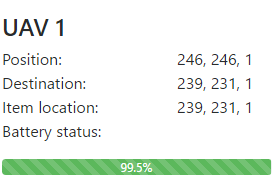
\includegraphics[scale=0.5]{images/uav_detail.png}
		\caption{Detailed view of UAV information}
	\end{figure}


\subsection{UAV}\label{sec:UAV}
\begin{enumerate}
	\item most important component, tried to make a realistic simulation of a UAV's components and behavior, excluding flight behavior
	\item UAV do not communicate with a central entity such as a control server organizing the flight traffic. UAV communicate with each other if they are in sensor range and only rely on their own sensors.
	\item Perceived World contains all cells that the UAV knows already. It stores information on obstacles. To improve performance, this is realized using dictionaries, one for each height level, mapping coordinates to information whether there is an obstacle on that field or not. For performance reasons, we decided against using MESA's grid here as iterating it reduces performance significantly. This is especially true for the grid exchange where each UAV  would have to check every field on the grid for content.  A dictionary contains unique values and is easier to exchange.
	\item Components: The simulated UAV has certain components that are taken from the real world:
	\begin{itemize}
		\item FlightController: This component contains the path-finding/route-planning algoritm. It represents a navigation unit. Multiple algorithms could be implemented, compare section \ref{sec:algorithm} for an example. The algorithm can make use of the exchanged information on the grid provided by the \textit{CommunicationModule} component and thus supports swarm algorithms.
		\item Battery: The battery has a limited battery life that decreases on each step. When the battery reaches a certain threshold (configurable), the UAV will fly to the nearest depot to recharge.
		\item CargoBay: The cargoBay represents the UAV's storage unit which can contain exactly one item.
		\item CommunicationModule: If the sensor found another UAV in the sensor's radius, this component will communicate with the other UAV and exchange grid information. Exchange of information on previously-unknown terrain helps when a UAV has to deliver an item to a new area of the map. This allows for precomputing optimal routes before exploring the actual area.
		\item Sensor: Scanning the grid for obstacles and other agents. This component is the interface to the model
	\end{itemize}
	\item States

\end{enumerate}


\cite{jang.2005} can be helpful to structure this part!


\begin{enumerate}
	\item multiple depots
	\item Describe the modular and extensible character of the architecture
	\item Describe how the model accomodates for the integration of self-organizing algorithms for UAVs
	\item Describing changes and extensions in the mesa framework
	\item drones have to recharge and thus deviate from their actual route
	\item ...
	
\end{enumerate}


\subsection{Analytics}\label{sec:KPI}
During a run, data and results are being generated. To allow for the evaluation of a path finding algorithm
For evaluating the delivery scenario, we identified the following KPI's:
\begin{itemize}
	\item Average walk length: Describes the average number of steps taken for an item to be delivered. 
	\item Average walk length divided by initial distance: This data point is a ratio calculated by dividing the average number of steps taken by the initial distance from base station to an item's destination. The initial distances are calculated as euclidean distances. Example: A value of 2 means that the average walk length is 2 times the initial distances.
	\item Standard deviation of average walk lengths: Represents the standard deviation of all walk lengths to get a better insight into the data additional to the average walk length.
	\item Items delivered per UAV: Items delivered divided by number of UAV's.
	\item Average lifetime of item: Calculation of the average lifetime of items by aggregating all item's lifetimes, divided by number of items. Lifetime is defined as the time from being available for delivery at the depot to the actual delivery at the item's destination.
\end{itemize}

The results are step-wise written out into a CSV file during the simulation and can for example be imported into a spreadsheet software or more sophisticated tools like R or any other application to run statistical analysis of the KPI's. Technically, this is realized by using MESA's DataCollector class. This allows for easy definition of values to be calculated every step and export them to a CSV file. The KPI's can easily be extended or modified in the source code.

\begin{figure}[htbp]
	\centering
	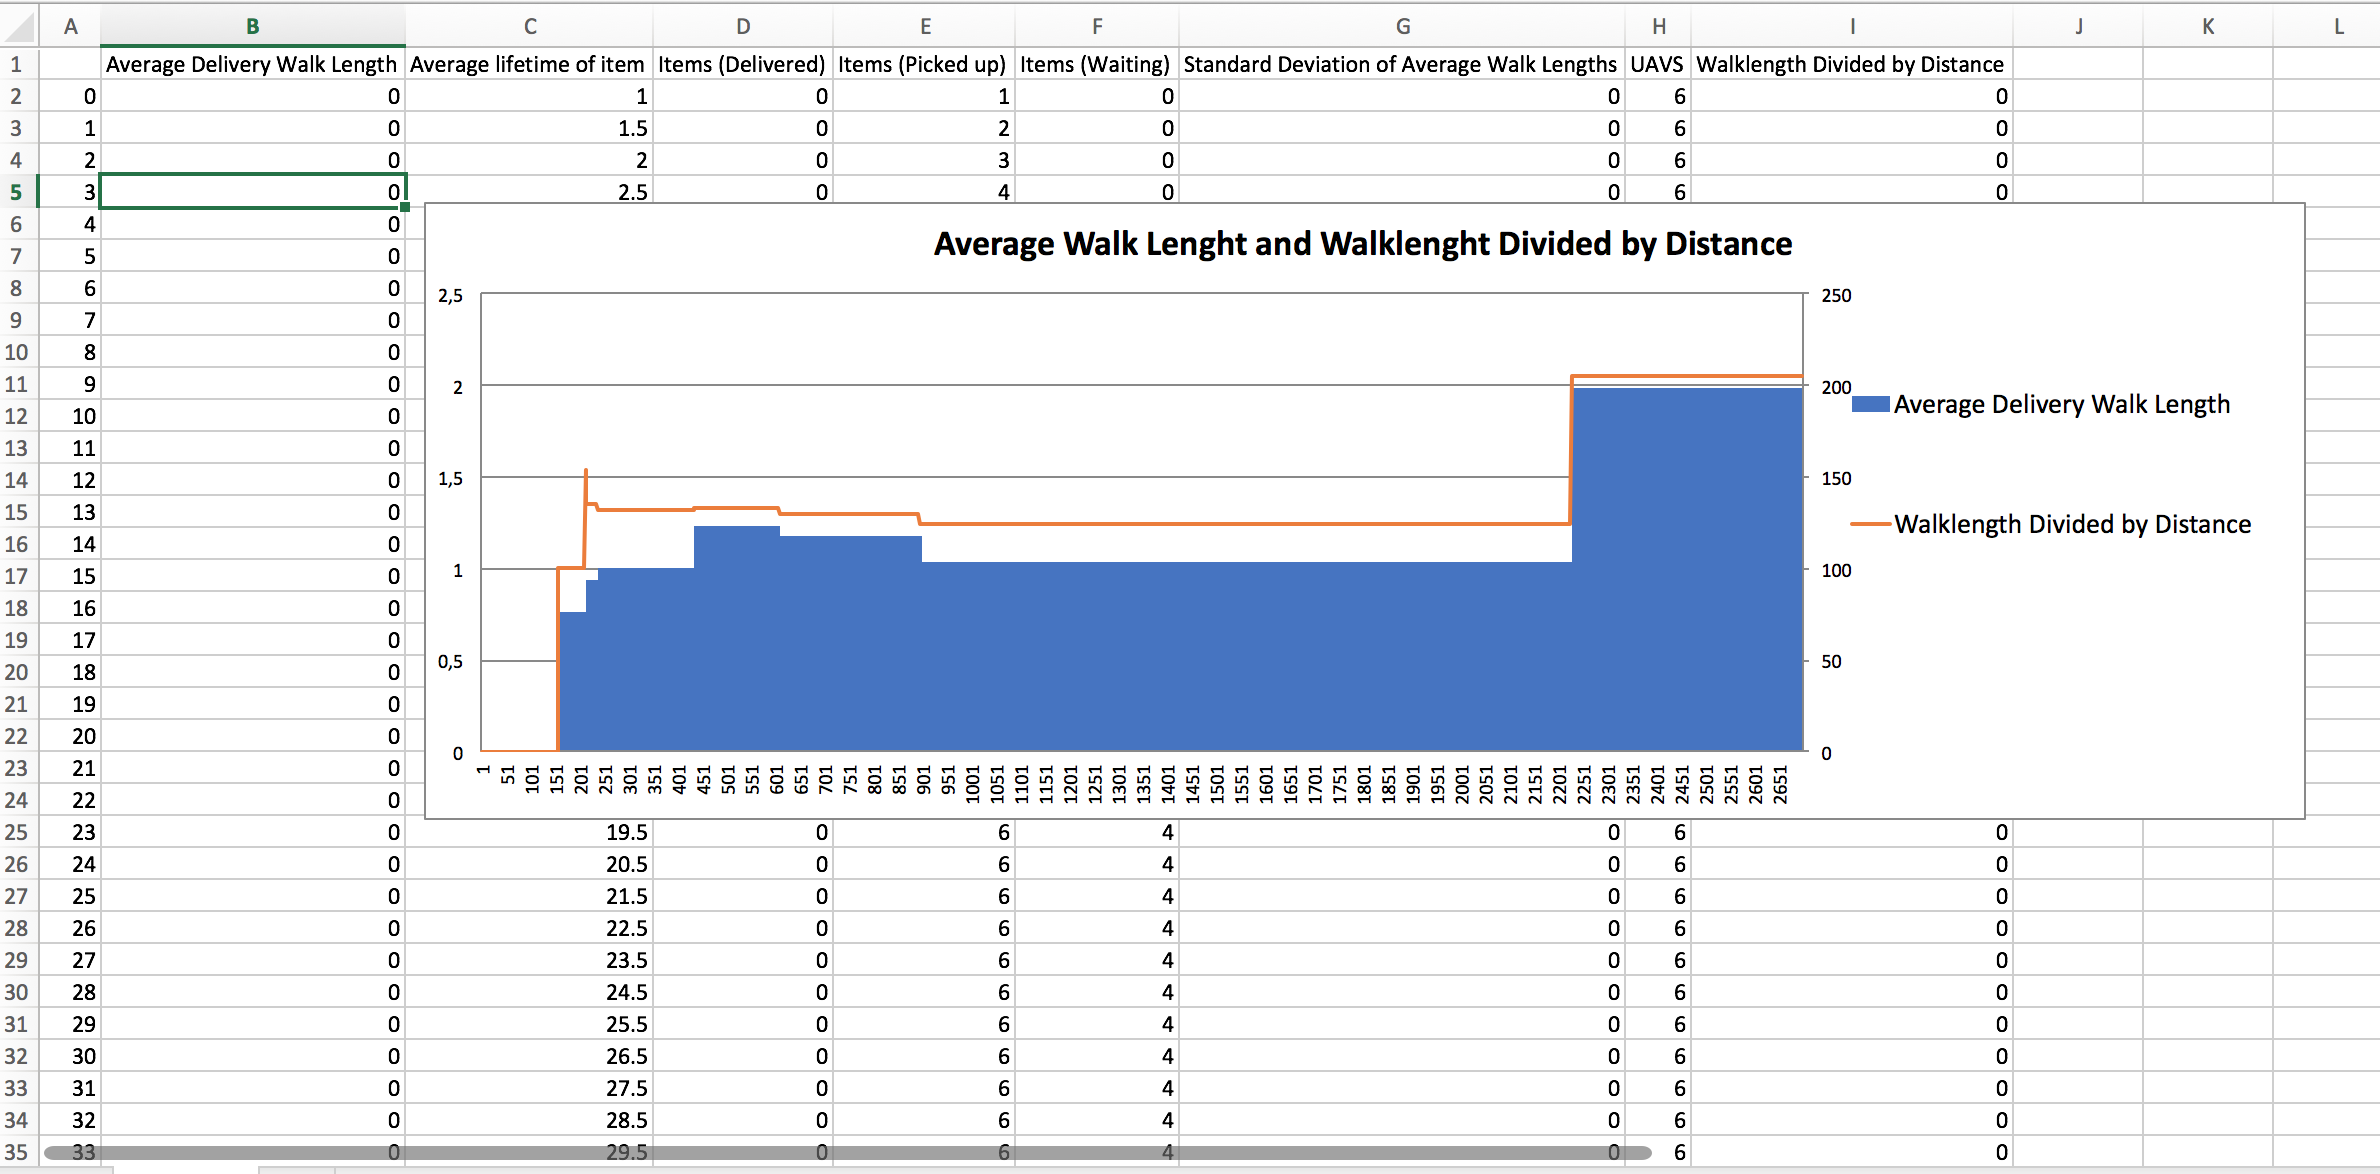
\includegraphics[scale=0.4]{images/walk}
	\caption{Example of analyzing KPI's in a spreadsheet software}
\end{figure}

\begin{itemize}
	\item KPI's
	\item out.csv
	\item DataCollector from MESA
	
\end{itemize}

\section{Implementation of a sample algorithm: A Star}\label{sec:algorithm}
To provide an example simulation, the A* algorithm has been used 
SOURCES!


\section{Evaluation}
NOT SURE WHAT TO WRITE HERE. ALGORITHM EVALUATION OR RATHER OUR TOOL? BUT THEN WHAT TO EVALUATE? PERFORMANCE? \\
The simulation engine presented in this paper allows for a simple evaluation of a path planning algorithm in a 3-dimensional space. Also it helps to implement traditional algorithms into a swarm optimization problem as UAVs exchange their grid whenever they come close enough to each other. A bottleneck is the calculation performance. On a mid-2015 Macbook Pro with a i5 Dual core processor, the simulation of 5000 steps (run without GUI) still takes a very long time. This is due to the fact that the implementation of the MESA grid used in the model is not very performance-optimized. Also, the exchange of the grid is a complex task. It was tried to optimize performance by using dictionaries for the grid's perceived world rather than storing a complete grid. The model's internal grid also has been modified to just store values for obstacles (1+altitude), baseStations/depots (-1) or 0 for nothing. This step had a high impact on performance but optimizing the complexity in an algorithm's calculations is the programmer's task.

\section{Conclusion}
\begin{enumerate}
	\item Overall summary
	\item limitations of this approach
	\item future development?
\end{enumerate}

